\subsection{手写 RISC-V 汇编的组织与调用约定}
六组示例采用 RV64GC 指令集和 LP64D 调用约定。
整数参数和返回值使用 a0 等参数寄存器，浮点函数的单精度参数和返回值使用 fa0。
遵循 RISC-V psABI\cite{riscvabi}，函数调用处保持 sp 的 16 字节对齐，
使用 s 寄存器的函数保存并恢复相应值；非叶函数保存返回地址 ra。
跨调用保留的数据存入 s 寄存器或栈中。

\begin{table}[htbp]
\centering\small
\begin{tabular}{p{0.25\linewidth}p{0.62\linewidth}}
\toprule
文件 & 实现重点\\
\midrule
arithmetic\_rv.s & word 算术、向零截断除法、有符号余数、跨输出调用保存输入\\
short\_circuit\_rv.s & 受保护除法、分支短路、全局 hits 与 touch 副作用\\
loop\_control\_rv.s & continue 回边、break 出口、循环状态寄存器\\
functions\_rv.s & 递归栈帧、保存 ra 与原参数、void 输出函数\\
array\_float\_rv.s & 二维数组行步长、补零、float ABI、显式截断转换\\
promote\_demo\_rv.s & 寄存器求和循环，与内存形式 LLVM IR 对照\\
\bottomrule
\end{tabular}
\caption{手写汇编与同名 SysY、LLVM IR 示例的对应关系}
\end{table}

SysY 的 int 是 32 位，而 RV64 的整数寄存器是 64 位。
因此使用 addw、addiw、subw、mulw、divw、remw 等指令处理整数计算，
lw 读取数组元素，并保持 32 位结果的符号扩展。寻址和 sp 调整则使用 64 位指令。
伪指令 call、ret、li、la 由汇编器展开。

\subsection{短路、循环与递归的目标代码表达}
短路例子先检查 n，再进入右侧表达式。以下为受保护除法的完整控制片段：

\par\vspace{0.7\baselineskip}\noindent\begin{minipage}[t]{\linewidth}
\begin{lstlisting}
    li a0,0
    beqz s0,.Land_done
    li t0,12
    divw t0,t0,s0
    li t1,2
    slt a0,t1,t0
.Land_done:
    call putint
\end{lstlisting}
\end{minipage}\par\vspace{0.5\baselineskip}

其中 s0 保存 n。n=0 时直接跳过 divw；另一个逻辑或条件在 n=0 时直接进入真分支，
不会调用 touch。全局 hits 通过 la/lw/sw 访问，输出次数与 LLVM IR 版本一致。
循环例子用寄存器保存 i 与 sum，continue 跳回条件检查，break 跳到输出出口。
LLVM IR 中的 phi 对应不同路径对状态寄存器的更新。

本例用 t0 保存 i、t1 保存 sum，输入上限保留在 a0。
循环内不调用其他函数，因此这些寄存器在整个迭代过程中保持可用。
遇到 2 时直接回到条件检查，t1 不变；遇到大于 5 的值时跳到出口，
只在普通路径执行 addw。这与 IR 中 skip、break.test、accumulate 三条路径一一对应。
\begin{table}[htbp]
\centering\small
\begin{tabular}{llll}
\toprule
输入上限 & 实际累加项 & 输出 & 控制路径\\
\midrule
0 & 无 & 0 & 初始条件退出\\
2 & 1 & 1 & 跳过 2 后退出\\
5 & 1、3、4、5 & 13 & 正常条件退出\\
8 & 1、3、4、5 & 13 & 处理 6 时 break\\
\bottomrule
\end{tabular}
\caption{同一寄存器循环中的条件退出、continue 与 break}
\end{table}

递归 factorial 的非基本情形保存原参数和 ra，再调用自身，汇编与对应运行记录见图\ref{fig:recursive-rv}：


\begin{figure}[H]
\centering
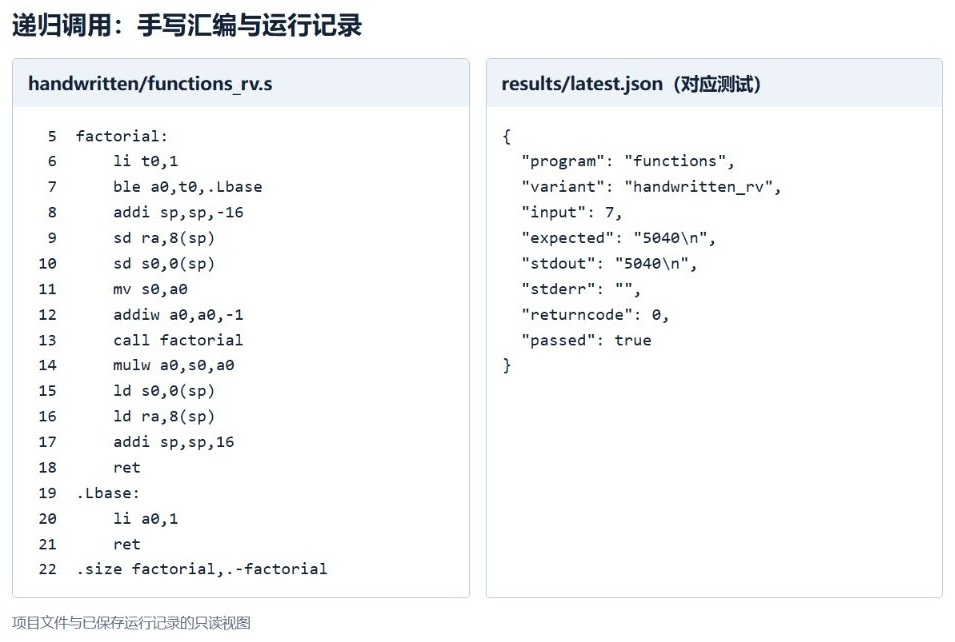
\includegraphics[width=\linewidth]{figures/recursive_rv.jpg}
\caption{递归阶乘的手写 RISC-V 汇编与输入 7 的测试记录截图}
\label{fig:recursive-rv}
\end{figure}


基本情形 n<=1 直接返回 1，不建立额外栈帧。
emit 不返回计算值，但它调用输出库，也必须保存 ra；源程序的 void 返回
对应恢复调用现场后 ret。测试 n=0、1、5、7、12，既检查递归出口也检查多层返回。

\subsection{栈帧布局与跨调用数据保存}
factorial 的非基例在 16 字节栈帧中保存 ra 和 s0，s0 持有当前层参数。
递归返回时 a0 已被子调用结果覆盖，所以乘法使用恢复前仍在 s0 中的原参数。
以 n=3 为例，子调用依次返回 1、2，当前层再计算 $3\times2=6$；
每层恢复 s0 和 ra 后释放自己的栈帧，使控制流返回正确的调用位置。

数组示例还需要在多次函数调用之间保存数组、浮点结果和中间整数。
其 main 实际使用如下 64 字节栈帧：
\begin{table}[htbp]
\centering\small
\begin{tabular}{lll}
\toprule
相对 sp 的偏移 & 宽度 & 用途\\
\midrule
0、4、8、12、16、20 & 各 4 字节 & 二维数组六个 i32 元素\\
24 & 4 字节 & scaled 的单精度值\\
28--39 & 12 字节 & 未用于保存有效数据的间隔\\
40、48 & 各 8 字节 & 保存 s1、s0\\
56 & 8 字节 & 保存 ra\\
\bottomrule
\end{tabular}
\caption{array\_float 的 main 栈帧布局}
\end{table}
调用 row\_sum 后，第一行结果转存 s0，随后第二次调用产生的 a0 与 s0 相加。
浮点结果提前用 fsw 保存到偏移 24，整数截断值放入 s1；
输出数组和整数后，再通过 flw 恢复浮点值完成正值判断。
这种安排使计算数据在所需调用期间保持有效，并在函数返回前恢复保存寄存器。

\subsection{数组布局与浮点数实现}
二维数组采用行优先布局，每行含三个 i32 元素，因此行步长为 12 字节。
row\_sum 接收 a0 中的数组首地址和 a1 中的行下标，用
$\mathrm{base}+12\times\mathrm{row}+4\times\mathrm{column}$ 计算元素地址。
main 的 64 字节栈帧中，偏移 0--20 保存六个元素，24 保存 scaled，
40、48、56 分别保存 s1、s0、ra；未初始化的两个数组元素显式写零。
输入和输出库调用使用独立栈帧，不覆盖调用者的数组区域。

整数输入通过 fcvt.s.w 转换为 float，fmul.s 与 fadd.s 计算
$1.5n+0.5$，twice 在 fa0 中收参并返回 $3n+1$。
fcvt.w.s 的 rtz 模式显式实现 float 到 int 的向零截断。
scaled 在后续 row\_sum、putint、putch 调用期间保存在栈上，
最后重新加载并用 flt.s 比较。

\subsection{手写与 LLVM 后端输出的对照}
验证过程同时保存 llc 生成的 O0、O2 汇编。
在 loop\_control 的 O0 文件中，循环状态使用 a0、a4、a5 等寄存器，
并形成 header.outer 与 body 对应的循环标签；
手写版本直接用 t0/t1 更新 i 与 sum，保留与源程序对应的标签。
O2 IR 则出现 body.peel、next.lcssa 等块和值，并在处理跳过 2 的路径上形成常量 3。
生成的目标代码因此不再逐块复刻原始手写 IR。

这一对照分为三个层次：先检查源语言的跳过与退出规则，再检查 IR 的合流值，
最后检查目标代码中的分支、寄存器更新和调用现场。
六组循环输入在原始 IR、O2 IR 和手写汇编路径上输出一致，
说明这些不同的代码组织保持了测试输入上的计算结果。

\subsection{汇编、链接和同输入等价性验证}
验证脚本对每个手写文件执行静态链接并由 QEMU 运行，例如：
\par\vspace{0.7\baselineskip}\noindent\begin{minipage}[t]{\linewidth}
\begin{lstlisting}[language=bash]
riscv64-linux-gnu-gcc -static -march=rv64gc -mabi=lp64d \
  prep/llvm_ir/handwritten/functions_rv.s prep/manual/sylib.c \
  -o build/prep-llvm-ir/functions_handwritten_rv
printf '7\n' | qemu-riscv64 build/prep-llvm-ir/functions_handwritten_rv
# stdout: 5040, process exit status: 0
\end{lstlisting}
\end{minipage}\par\vspace{0.5\baselineskip}
汇编器生成目标代码，链接器解析库函数，QEMU 执行 RV64 程序。

\begin{table}[htbp]
\centering\small
\begin{tabular}{llll}
\toprule
示例 & 代表输入 & 源程序/IR/手写汇编 stdout & 验证重点\\
\midrule
arithmetic & -7 & 1, 7, -7, -7 & 负数除法与余数\\
short\_circuit & 0 / 4 & 0, 2, 0 / 1, 2, 1 & 短路与副作用\\
loop\_control & 2 / 8 & 1 / 13 & continue / break\\
functions & 7 & 5040 & 递归与返回\\
array\_float & -3 / 2 & 10, -8, 0 / 10, 7, 1 & 数组、浮点与转换\\
promote\_demo & 5 & 10 & 循环累加\\
\bottomrule
\end{tabular}
\caption{实际执行的代表结果，逗号表示换行分隔的输出}
\end{table}

每个输入比较八条路径：C 参考程序本机/RV64、手写 IR 本机/RV64
（原始与 O2）、lli、手写 RV64 汇编。33 组输入共 264 项，
加 mem2reg 的 5 项为 \textbf{269/269 通过}。
arithmetic、short\_circuit、loop\_control 各 48 项，functions 与 array\_float 各 40 项，
promote\_demo 含 mem2reg 共 45 项。全部输出逐字比较，并检查进程退出码为 0。
